\section{Optical MIMO system with imaging receiver}
\label{sec:mimoImaging}

\subsection{Optical imaging MIMO channel}
\label{subsec:mimoImagingChannel}

\graphicspath{{_MIMOSpace/figures_mimoImg/}}
In this section, an optical MIMO imaging system as illustrated in \figurename{ \ref{figMIMOblock}} is considered. Multiple luminaires are located near the ceiling of an indoor space to provide illumination and act as transmitters for communication. Information to transmit is jointly coded across a set of luminiares within the FOV of the receiver. User requested illumination state sets the average radiant flux emitted by the transmitters. Based on these inputs, the modulator generates drive signals for each luminaire. LEDs in the luminaire convert modulated data in the electrical domain into optical signals in the visible spectrum (E/O and conversely O/E conversion). These optical signals propagate through the indoor space and are incident on the receiver. 

\begin{figure}[!t]
	\centering
		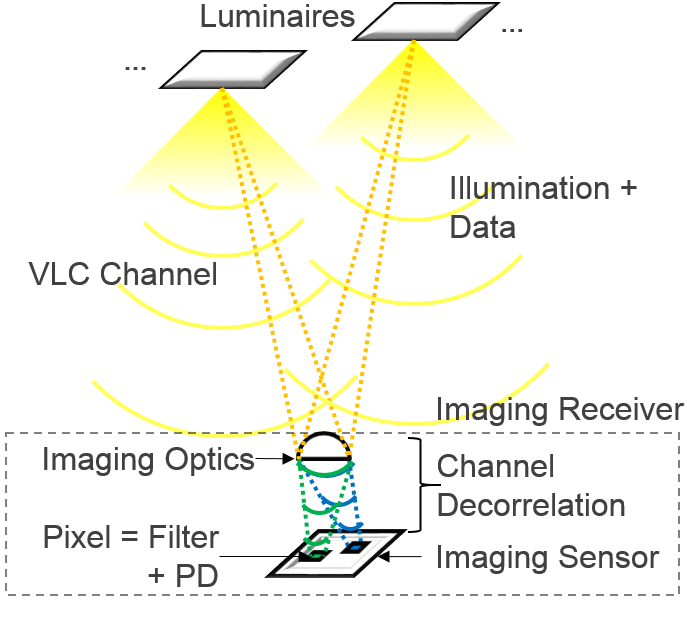
\includegraphics[trim={0.5in 0.25in 0.5in 0.25in}, clip=false, width=3.2in]{figMIMOmodel2.png}
	\caption{Optical MIMO system with imaging receiver}
	\label{figMIMOblock}
\end{figure}

\figurename{ \ref{figImagingReceiver}} illustrates a schematic of an imaging receiver. An imaging receiver for OWC can be modeled as a sensor and imaging optics. The sensor is located at a distance $f$ away from the optical center of the lens and is comprised of a grid of detector elements - each referred to as a `pixel'. Each pixel is comprised of a filter and optical detector. The imaging optics redirect light rays originating from different of an irradiating planar surface such that they are incident on corresponding different locations on the sensor. In other words, based on the angle and the location of incidence, light rays are redirected by the imaging optics on to a specific path. Thus it can extract and isolate optical signals originating from different spatial locations that get mixed while propagating through the indoor space. This helps to decorrelate signals received from spatially distinct transmitters and help significantly improve communication performance. Similarly, the ambient radiant flux incident at the aperture of the receiver is distributed among all pixels of the sensor. This helps to significantly reduce shot noise per pixel \cite{dja00a}. The receiver uses all received streams to jointly decode and recover information. 

\begin{figure}[!t]
	\centering
		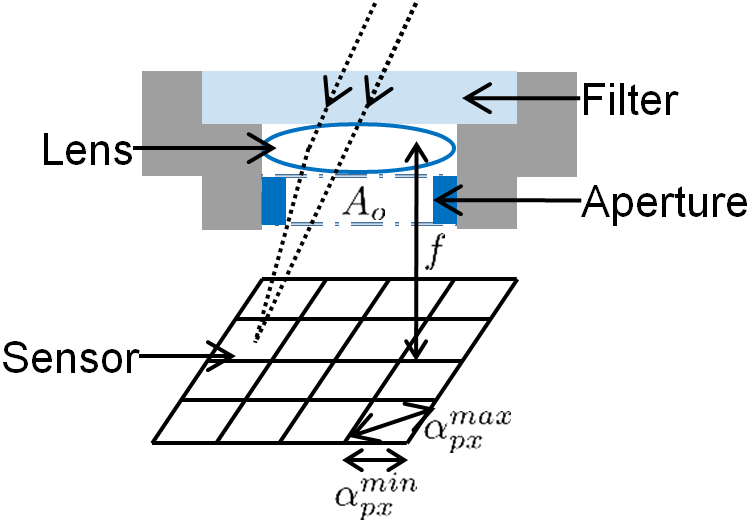
\includegraphics[width=3in]{figImagingReceiver.png}
	\caption{Schematic of an imaging receiver}
	\label{figImagingReceiver}
\end{figure}

Let $N_{\text{tx}}$ represent number of luminaires using which information is transmitted to user and let $N_{\text{px}}$ represent number of contiguous pixels comprising the sensor of an imaging receiver. The optical $N_{\text{tx}} \times N_{\text{px}}$ MIMO system can be represented by
\begin{equation}
	\label{eqMimoChannel3}
	\bf{Y} = \bf{H}\bf{X} + \bf{W}
\end{equation}
$\bf{X}$ is a $N_{\text{tx}}$ dimensional vector whose each element is the signal radiant flux emitted by each transmitter. The flux propagates over multiple paths before being incident on the imaging optics. As discussed in the SISO system, the LOS component of received flux is dominant over the NLOS component due to additional propagation and non--ideal reflection losses . $\bf{H}$ is a $N_{\text{px}}\times N_{\text{tx}}$ dimensional channel gain matrix where each element or channel gain coefficient $h_{ij}$ indicates the net channel gain from transmitter $j$ to pixel $i$. $\bf{W}$ is a $N_{\text{px}}$ dimensional noise vector. For imaging receivers, the shot noise at each pixel due to ambient illumination is severely diminished \cite{dja00a} and thus TIA input noise current is dominant source of noise \cite{kah97a}. For imaging receivers, ${\bf{W}}\sim\mathcal{N}({\bf{0}}$, $\sigma_{n}^2{\bf{I}})$ where $\sigma_{n}^{2}$ equals total noise current density. $\bf{Y}$ is a $N_{\text{px}}$ dimensional vector whose each element is the output signal current from each pixel.

For each individual link between transmitter $j$ and pixel $i$, the free space gain is defined as the fraction of the radiant flux emitted by the transmitter that is incident on the receiver aperture. Let [$x_{j}$ $y_{j}$ $z_{j}$] be the location of centroid $C_{j}$ of the illumination surface of the $j^{th}$ transmitter and [$x_{\text{rx}}$ $y_{\text{rx}}$ $z_{\text{rx}}$] be the location of the centroid of the receiver aperture. Optical axis ($\vm{d}_{j}$) between transmitter $j$ and receiver can be computed from Eq. \eqref{eqOpAxis}. The free space channel gain is then given by
\begin{equation}
	\label{eqMimoHFS}
	h^{\text{fs}}_{j} = L_{j}(\phi_{j})\frac{A_{\text{o}}}{||{\bf{d}}_{j}||^2}cos(\psi_{j})
\end{equation}
$\phi_{j}$ is the angle subtended between the optical axis and surface normal of the transmitter. $L_{j}(.)$ is the Lambertian radiant intensity as given by Eq. \eqref{eqLambertian}. Let $A_{\text{o}}$ be the area of the aperture opening. $\psi_{j}$ is the angle between the optical axis and surface normal of the receiver.

The magnification property of imaging optics determines the point of incidence on the sensor for a ray of light originating from the irradiating surface of the transmitter. Using ray tracing methods for a point aperture, it can be mathematically represented by
\begin{equation}
	\label{eqOpMag}
	M_{\text{im}} = \twopartdef {\frac{f}{||{\bf{d}}_{j}^{z}||-f}} { \psi_{j}\leq\psi_{c}^{rx}} {0} { \psi_{j}>\psi_{c}^{rx}}
\end{equation}
$f$ is the focal length of the imaging optics. $\psi_{c}^{rx}$ is the FOV of the receiver. Depending on the sensor dimensions, this may be smaller than or equal to the FOV of imaging optics.
Assuming the receiver is focused on the transmitter, the location of $C_{j}$ as projected in the RCS is given by
\begin{equation}
	\label{eqLocSp}
	{\vectthree{x_{\text{sp}}}{y_{\text{sp}}}{z_{\text{sp}}}}_{j} = \vectthree{-M_{\text{im}}({\bf{d}_{j}}.{\hat{\bf{x}}})}{-M_{\text{im}}({\bf{d}_{j}}.{\hat{\bf{y}})}}{-f}
	\end{equation}
	
Assuming the mathematical model of the shape of the luminaire's illumination surface is known, the shape of its projected spot on the plane of surface of the sensor can be calculated. Depending on the geometry of the transmitters and receiver, a pixel may receive light from multiple spots. Accordingly, the system performance gets severely degraded due to  the correlated channel matrix coefficients and inter channel interference (ICI). Non-polygonal shapes can be approximated to a polygon with very small error. Polygon itersection algorithms can be used to compute the shared area between a spot and pixel. The imaging channel gain (\ref{eqMimoHIm}) between transmitter $j$ and pixel $i$ is then given by the ratio of the fraction of the area of the spot $j$ that is incident on pixel $i$ to total area of the spot $j$.
\begin{equation}
	\label{eqMimoHIm}
	h^{\text{im}}_{ij} = \frac{\text{Area}(\text{spot}_{j}\cap \text{pixel}_{i})}{\text{Area}(\text{spot}_{j})}
\end{equation}
%\begin{equation}
	%\label{eqMimoHIm}
	%h^{\text{im}}_{ij} = \twopartdef{1}{\text{ spot$_{j}$ inside pixel i}}{0}{\text{ otherwise}}
%\end{equation}

Let $S_{j}(\lambda)$ be the SPD of the flux over link $j$ and $T_{i}(\lambda)$ and $R_{i}(\lambda)$ be the filter transmittance and responsivity at pixel $i$ respectively. The optical filter transmittance in this case is assumed independent of the angle of incidence of the flux. Let $Q$ be the transmittance of the imaging optics. The effective responsivity of pixel $i$ over link $j$ is given by
\begin{equation} 
	\label{eqPxResp}
	R_{ij} = Q\int_{\lambda_{min}}^{\lambda_{max}}S_{j}(\lambda)T_{i}(\lambda)R_{i}(\lambda)d\lambda
\end{equation}

Thus the net channel gain matrix $\bf{H}$ can be computed from the free space channel gain, the imaging channel gain and effective pixel responsivity by
\begin{equation}
	\label{eqMimoH}
	{\bf{H}}(i,j) = h_{ij} = h^{\text{fs}}_{j}h^{\text{im}}_{ij}R_{ij}
\end{equation}
where element $h_{ij}$ is the net channel gain from transmitter $j$ to pixel $i$.

